\documentclass[a4paper, ngerman,12pt]{scrartcl}
\usepackage[backend=biber]{biblatex}
% TODO: [ ] Was ist eine REST-API
% Setup {{{1
% Packages {{{2
%\usepackage[margin=1in]{geometry}
\usepackage{amsfonts, amsmath, amssymb}
\usepackage{babel}
\usepackage{graphicx}
\usepackage{float}
\usepackage[utf8]{inputenc}
\usepackage{fancyhdr}
\usepackage{tikz}
\usepackage{csquotes}
\usepackage{xpatch}
\usepackage[gen]{eurosym}
\usepackage{mathptmx}
\usepackage[scaled=0.9]{helvet}
\usepackage{courier}
\usepackage[T1]{fontenc}
\usepackage[breaklinks=true]{hyperref}
\usepackage{wrapfig}
\usepackage[onehalfspacing]{setspace}
% Heading {{{2
\pagestyle{fancy}
\fancyhead{}
\fancyfoot{}
\fancyhead[L]{\slshape \MakeUppercase{Informatik Jahresarbeit}\/}
\fancyhead[R]{\slshape Jasper Levin Spahl\/}
\fancyhead[C]{\thepage}
% Paragraph {{{2
%\parindent 0ex
\setlength{\parindent}{1em}
\setlength{\parskip}{1em}
\renewcommand{\baselinestretch}{1.1}
% }}}
\author{Jasper Levin Spahl}
% Tikz Setup {{{2
\usetikzlibrary{shapes.geometric, arrows.meta}
% Bibliograthy Setup {{{2
\addbibresource{quellen.bib}
\begin{document}
% Titlepage {{{2
\begin{titlepage}
\begin{center}
\vspace*{1cm}

\Large{\textbf{Informatik}}\\
\Large{\textbf{Jahresarbeit}}\\
\vfill
\line(1,0){400}\\[1mm]
\huge{\textbf{Der Smarte Bienenstock}}\\[3mm]
\Large{\textbf{- 12 Kss -}}\\
\line(1,0){400}\\
\vfill
Jasper Levin Spahl\\
Klasse: 12Kss\\
\today\\
\end{center}
\end{titlepage}

% Table of contents {{{2
\tableofcontents
\thispagestyle{empty}
\clearpage
\setcounter{page}{1}

% Einleitung {{{1
\section{Einleitung}

Bei der Auswahl des Themas meiner Jahresarbeit war ich lang unentschlossen.
Ich wusste sofort, dass ich entweder etwas kreatives oder etwas Im It-Bereich machen wollte.
Meine erste Idee war es einen Lichtwecker zubauen.
Ich bemerkte jedoch als ich damit fast fertig war das, dass ganze sehr viel leichter umzusetzen war, sodass ich damit keine komplette Jahresarbeit füllen konnte.
Mir gefiel allerdings das Thema Smarthome/Homeautomation.
Letztendlich brachte mich mein Vater auf die Idee.
Er erzählte mir vom einem Freunde der eine Bienenstockwaage besitzt.
Mit hilft so einer Bienenstockwaage kann man überwachen wie viel Honig sich gerade in dem Stock der auf ihr steht befindet.
Diese Waagen kosten zwischen 800 und 3000 \euro{}, sind somit viel zu überteuert.

Wenn man jedoch eine billigere Version haben will muss man sie sich selbst bauen.
Es gibt zwar, wie ich später herausfand, eine relative einfache Bauanleitung für ein solches System.
~\cite{Honeypi}
Allerdings benötigt dieses System einen Anschluss an eine Cloud, dessen Source Code nicht offen ist.
Das heißt die Daten werden an irgendeinen Server übermittelt der sie dann speichert.
Man weiß also nicht er alles auf die Daten zugreifen kann.
Diese potenzielle Sicherheitslücke hat man nicht, wenn man das ganze selbst entwickelt.

% Wichtige Begriffe {{{1
\section{Wichtige Begriffe}
Da ich in meiner Jahresarbeit mit über komplexere Konzepte ist diese kurze Begriffserklärung notwendig.

% Was ist ein Server? {{{2
\subsection{Was ist ein Server?}
Der Begriff \enquote{\textbf{Server}} (englisch für \textit{Diener}) hat zwei Bedeutungen.
Es gibt Hardware und Soft\-ware-Ser\-ver.
Als \textbf{Soft\-ware-Ser\-ver} bezeichnet man ein Programm das einen speziellen Dienst anderen Programmen, sogenannten Clients (englisch für \textit{Kunden}), zur Verfügung stellt.
Ein Webserver zum Beispiel stellt eine Internetseite ins Netz.~\cite[ver.][]{IonosServer}

Wenn die meisten Leute an einen Server denken, haben sie einen große Server Farm im Kopf.
Doch ein Hard\-ware-Ser\-ver muss nicht unbedingt groß sein und viel Strom verbrauchen.
Ein \textbf{Hard\-ware-Ser\-ver}, auch \textit{Host} genannt, definiert sich dadurch das auf ihm einer oder mehrere Soft\-ware-Ser\-ver laufen. Das heißt jeder Computer, jedes Smartphone kann ein Server sein.
Selbst einen modernen Kühlschrank kann man heute zu tage als Server bezeichnen solange er eine Serversoftware benutzt um z.B. dir zu zeigen was du alles bei deinem nächsten Einkauf mitbringen musst.

% Was ist eine API {{{2
\subsection{Was ist eine API?}\label{sec:api}

Eine \textbf{API}, kurz für \enquote{\textbf{Application Programming Interface}}\footnote{englisch für \textit{An\-wen\-dungs\-pro\-gram\-mier Schnittstelle}}, ist eine Schnittstelle die es Programmen und Hardware ermöglicht mit einander zu kommunizieren.
Eine API kann von Anwendungsbereich zu Anwendungsbereich komplett verschieden sein.~\cite[][]{GSApi}


Es gibt viele veschidene Standarts eine API zu programmieren.

In meiner Jahresarbeit werde ich vorallem über \textbf{Web-APIs} reden.

% Funktionsweise meiner Bienenstockwaage {{{1
\section{Funktionsweise meiner Bienenstockwaage}

Eine Bienenstockwaage ist eigentlich recht simpel.
Im Grunde ist es nur eine Waage welche ihre Werte in regelmäßigen abständen speichert bzw.
mit Hilfe von SMS oder Internet an den Betreiber übermittelt.

\begin{figure}[ht]
	\centering
	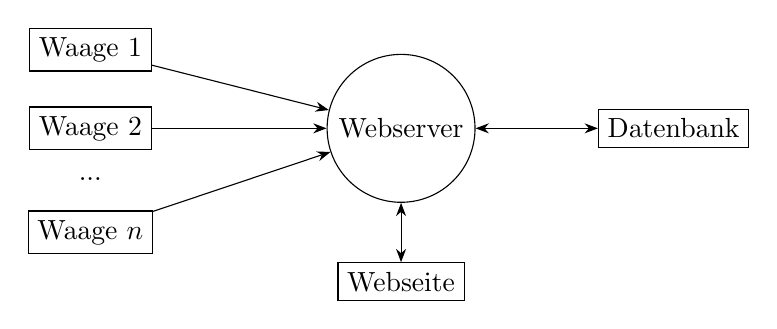
\begin{tikzpicture}

		\node[draw] (waage1) at (0,0) {Waage 1};
		\node[draw] (waage2) [below of = waage1] {Waage 2};
		\node[draw=none] (waage3) [below of = waage2, below = -0.5cm] {...};
		\node[draw] (waagen) [below of = waage3, below = -0.6cm] {Waage $n$};
		\node[draw, shape=circle] (server) [right of = waage2, right = 2cm] {Webserver};
		\node[draw] (app)    [below of = server, below = 0.7cm] {Webseite};
		\node[draw] (data)   [right of = server, right = 1.5cm] {Datenbank};

		\draw[-Stealth] (waage1) -- (server);
		\draw[-Stealth] (waage2) -- (server);
		\draw[-Stealth] (waagen) -- (server);
		\draw[Stealth-Stealth] (server) -- (data);
		\draw[Stealth-Stealth] (app) -- (server);
	\end{tikzpicture}
	\caption{Netzwerk Diagramm meines Serversystems\label{abb:networkdiagram}}
\end{figure}

Im Falle meiner Bienenstockwaage habe ich einen mir ein System überlegt, das gut skalierbar ist.
Dieses System besteht aus mehreren Bestandteilen welche über verschiedene APIs mit einander kommunizieren.

Das wichtigste Element davon ist der Hauptserver auf dem die Datenbank MongoDB und der Webserver laufen.
Ich habe mir dafür einen Raspberry Pi 3B+ angeschafft, da ich alle Daten lokal speichern wollte.
Das muss man aber nicht, da mach sich auch über die Plattform \href{https://www.mongodb.com/cloud/atlas}{MongoDB Atlas} eine Datenbank mieten kann und mit Hilfe von \href{https://www.linode.com}{Linode} oder \href{https://www.digitalocean.com/}{Digital Ocean} den Webserver hosten kann.

Die Datenbank kann man sich wie einen Schrank vorstellen in Ordner (Collections) sind worin sich Dokumente befinden.

Der Webserver hat zwei wichtige Aufgaben:
die Bereitstellung der Webseite und die Verwaltung der Daten.

In Abbildung~\ref{abb:networkdiagram} ist dieses da gestellt.


Wenn man sich die Daten anschauen will, kann man dies über eine Webseite die mit Hilfe einer REST-API
\footnote{Was eine REST-API ist können sie in Abschnitt~\ref{sec:api} lesen.}
mit dem Server verbunden ist.

% Literaturverzeichnis {{{1
\printbibliography{}
\end{document}
